\documentclass{article}
\usepackage[utf8]{inputenc}
\usepackage[T1]{fontenc}
\usepackage{graphicx}
\usepackage{hyperref}
\usepackage{geometry}
\geometry{margin=1in}

\title{BOTANY and HERBAL ANATOMY (Plate XLVI)}
\date{Encyclopaedia Britannica (1771)}

\begin{document}
\maketitle

\section*{Historical source}
\textbf{Entry ID:} \texttt{entry-britannica-volume-144133901-row-2209-2209} \\
\textbf{Volume ID:} 144133901 \\
\textbf{Character Count:} 800

\subsection*{Extracted Text}
Plate. XLVI B U X ( 697 ) B Y Z Button attempted to find out a north-well pallage to the Call Indies. It lies between 80° and 100° W, long, and between 60° and 60° N. lat.

[HISTORICAL COPPERPLATE ENGRAVING: BOTANY and HERBAL ANATOMY (Plate XLVI)]
Category: Botany and Plant Morphology
Visual Description: Detailed botanical copperplate engraving detailing plant reproductive organs, Linnaean floral classification components, stamen and pistil dissections, and seed capsule morphology.
Identified Engraved Figures:
  * Fig. 1: Complete floral dissection showing calyx, corolla, and stamens
  * Fig. 2: Pistil, style, and ovary cross-section revealing ovules
  * Fig. 3: Dehiscent seed capsule and cross-section
Related Scientific Subjects: Botany, Plant morphology, Linnaean taxonomy, Flower anatomy

\subsection*{Matched Wikipedia Article}
\textbf{Title:} History of the Encyclopædia Britannica \\
\textbf{Page ID:} 9004976 \\
\textbf{Revision ID:} 1340071003 \\
\textbf{URL:} \url{https://en.wikipedia.org/wiki/History\_of\_the\_Encyclop\%C3\%A6dia\_Britannica}


\section*{Source record}
\begin{itemize}
\item \textbf{Dataset:} \texttt{NationalLibraryOfScotland/encyclopaedia\_britannica\_illustrated}
\item \textbf{Dataset Revision:} \texttt{309f765b1ecc83e0a7f7762e44b4a927a7555443}
\item \textbf{Page ID:} \texttt{britannica:309f765b1ecc83e0a7f7762e44b4a927a7555443:train:2209} \\
  \textbf{Filename:} \texttt{page-2209-1ee9bc409f67.jpg} \\
  \textbf{Row Index:} 2209 \\
  \textbf{SHA256:} \texttt{1ee9bc409f6798b0...}
\item \textbf{Page ID:} \texttt{britannica:309f765b1ecc83e0a7f7762e44b4a927a7555443:train:2250} \\
  \textbf{Filename:} \texttt{page-2250-75315f455009.jpg} \\
  \textbf{Row Index:} 2250 \\
  \textbf{SHA256:} \texttt{75315f45500988da...}
\end{itemize}

\begin{figure}[h]
\centering
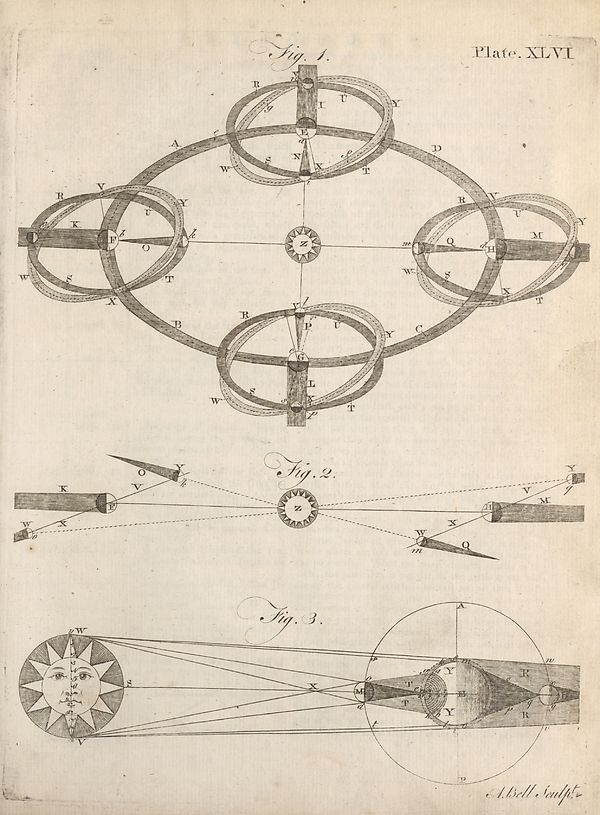
\includegraphics[width=0.85\textwidth]{../scans/page-2209-1ee9bc409f67.jpg}
\caption*{Source scan: \texttt{page-2209-1ee9bc409f67.jpg}}
\end{figure}
\begin{figure}[h]
\centering
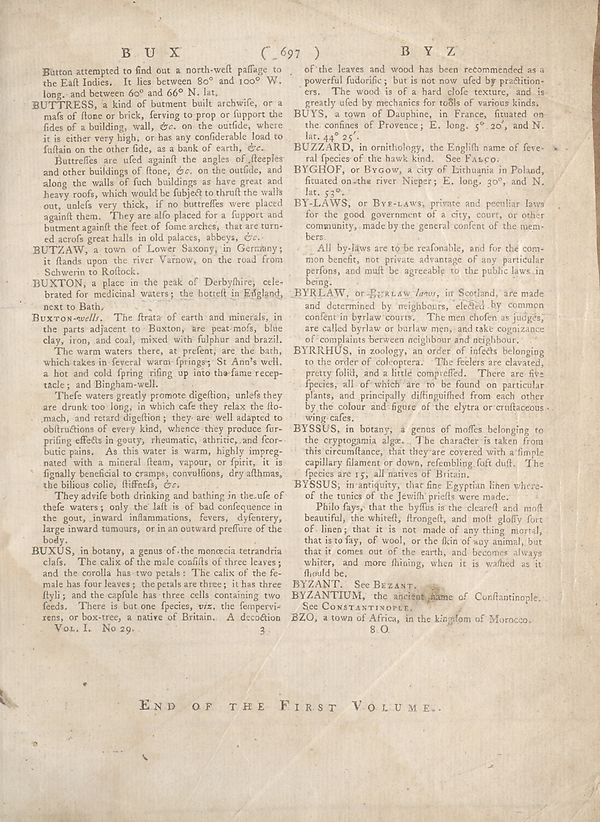
\includegraphics[width=0.85\textwidth]{../scans/page-2250-75315f455009.jpg}
\caption*{Source scan: \texttt{page-2250-75315f455009.jpg}}
\end{figure}

\end{document}
